\documentclass[UTF8]{ctexart}
\usepackage{graphicx}
\usepackage{amsmath}
\begin{document}
\section{非常数截面}
设粒子运动过程中的流强$I(x)$,对于经过薄层后的衰减为
\[dI=-\frac{I}{l(x)}dx\]
那么左右积分可以得到
\[I=I_0e^{-\int_0^x{\frac{1}{l(x)}dx}}\]
\section{模拟粒子碰撞}
二维散射,湮灭过程A,B.其中$l_s=0.1m,l_A=5m,l_B=0.3m$,特别注意散射后的角度在$[-30\deg,30\deg]$变化。
\subsection{模拟径迹图}
100个粒子在二维平面内的径迹如图所示,其中假定了初始出射方向向右:
\begin{figure}[h]
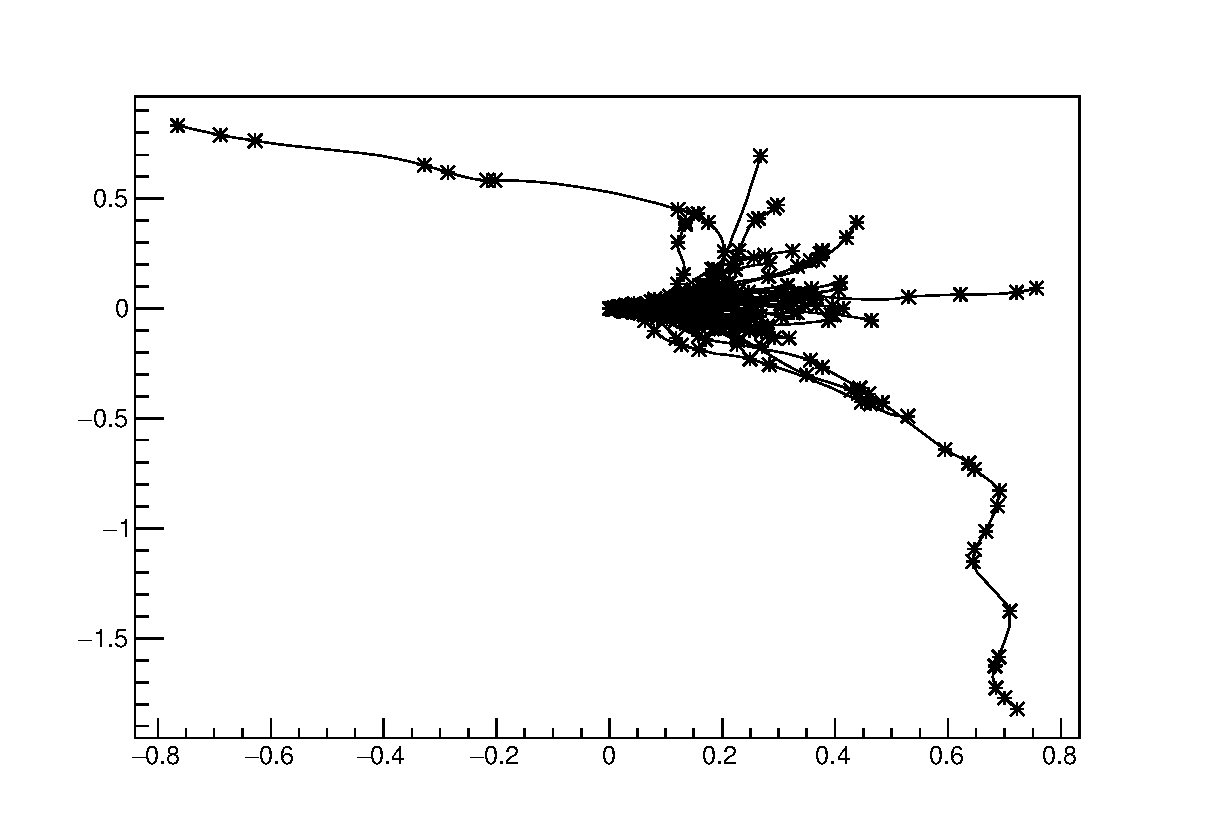
\includegraphics[width=.8\textwidth]{track100.eps}
\end{figure}
\subsection{模拟自由程分布}
湮灭A和湮灭B的平均路程分布如下图所示:
实际绘制过程中向histogram中加入每次track的总长度,然后画出对应的分布图。这个分布图代表在湮灭过程A,B过程的影响下,粒子行走的长度。
\begin{figure}[h]
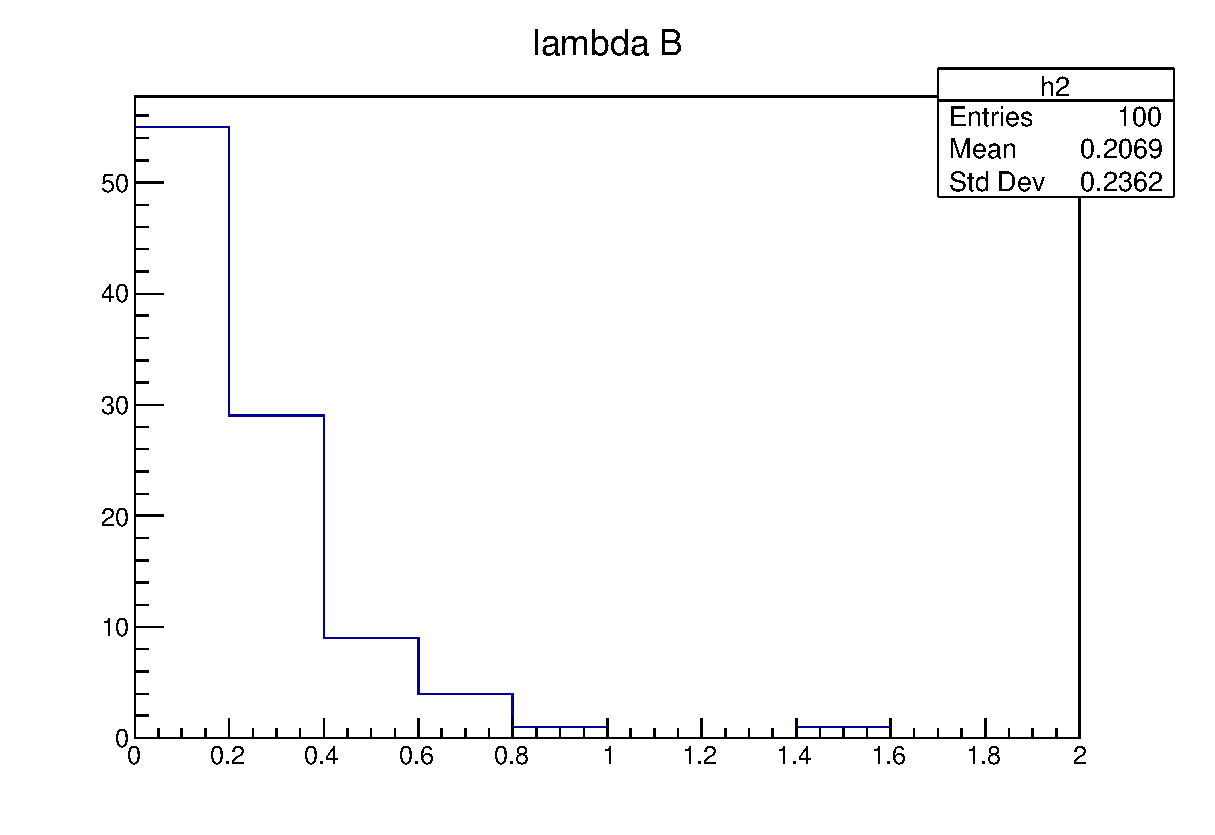
\includegraphics[width=.8\textwidth]{distribution100.eps}
\end{figure}
对于模拟结果$\lambda=0.20m$
\subsection{理论计算}
首先出发点是经过$x$距离后剩余概率是
\[P(x)=e^{-x/l}\]
那么对于有两种湮灭过程的散射,剩余概率应该是两者乘积
\[P(x)=e^{-x/l_1}e^{-x/l_2}\]
把上式化简之后就可以得到新的湮灭长度为下面式子:

理论计算应该为$\lambda=\frac{1}{\frac{1}{\lambda_A}+\frac{1}{\lambda_B}}=\frac{1}{\frac{1}{5}+\frac{1}{0.3}}=0.28m$
发现比理论计算小了一些,在写代码过程中有一个地方并没有考虑很恰当,算出湮灭概率更大后是应该立刻湮灭还是行走一段散射距离。

仔细考虑后,应该还是要再行走一段距离,因为这个模拟本质上是用散射距离来分割每次过程,判断是否湮灭,所以每一段应该都要加上才对。

重新模拟结果为$\lambda=0.40m$,和理论仍有差距。因为此时我加上的是散射距离。

此处感谢\texttt{杨宇祺}同学的指点,最后一段加入的应该是湮灭距离,也就是最小的距离,而不应该全部使用散射距离,因为本来湮灭就停止了,肯定不应该接着用散射距离来算。此时模拟结果为$\lambda=0.22m$.

\begin{figure}[h]
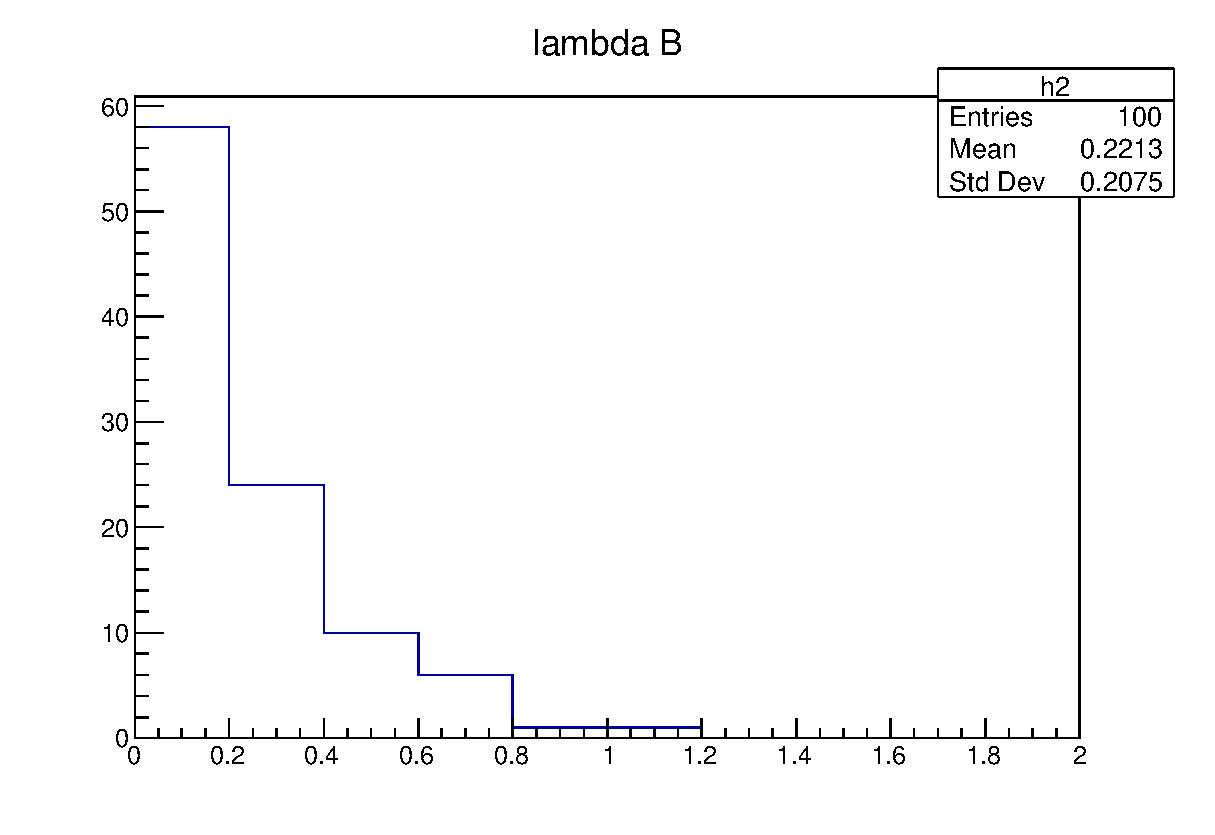
\includegraphics[width=.8\textwidth]{distributionN100.eps}
\end{figure}

个人认为这个问题出在如何考虑最后湮灭的一步时加入的长度。

再次增加模拟数量,模拟结果为$\lambda=0.28m$,和理论结果符合的很好。

\begin{figure}[h]
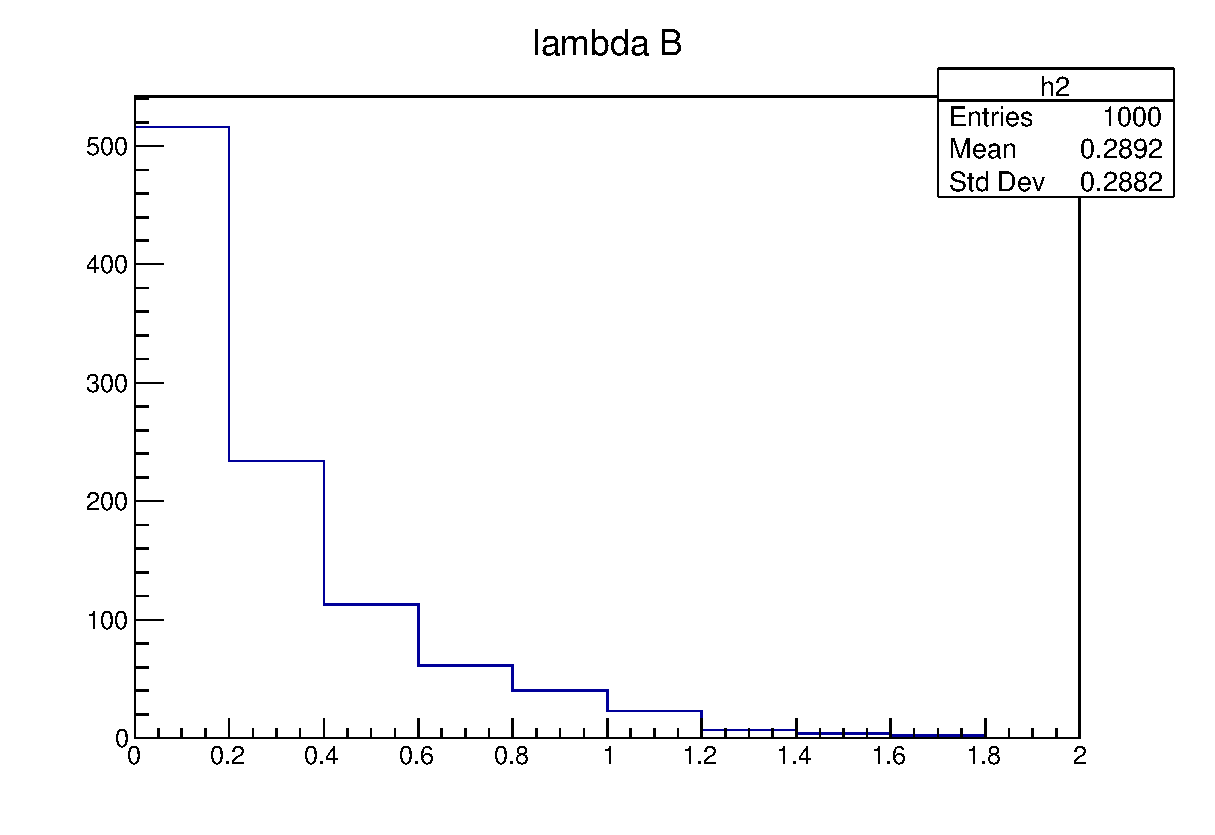
\includegraphics[width=.8\textwidth]{distributionN1000.eps}
\end{figure}
\end{document}
